\documentclass[]{beamer}
\usefonttheme{professionalfonts}
% Class options include: notes, notesonly, handout, trans,
%                        hidesubsections, shadesubsections,
%                        inrow, blue, red, grey, brown

% Theme for beamer presentation.
\usepackage{beamerthemetree} 
% Other themes include: beamerthemebars, beamerthemelined, 
%                       beamerthemetree, beamerthemetreebars  

\title{Orbital Optimization in Valence Bond Theory}
\author{Jeroen Engelberts}
%\institute{SURFsara}
\date{9 September 2013}

\begin{document}

\begin{frame}
  \titlepage
\end{frame}

\begin{frame}
  \frametitle{Goal}
  Analyze the orbital optimization process in the Valence Bond Self Consistent Field (VBSCF) method and look for possibilities to improve the performance, \textit{i.e.} decrease the computation time.
\end{frame}

\begin{frame}
  \tableofcontents
\end{frame}

\section{Valence Bond Theory}

\subsection{Valence Bond Wave Functions}

\begin{frame}
  \frametitle{Single Structure Wave Function}
  \begin{center}
    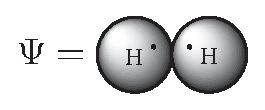
\includegraphics{figures/heitler.eps}  
  \end{center}
  \begin{equation*}
    \Psi = N \{ |1s_{A}\overline{1s_{B}}| - |\overline{1s_{A}}1s_{B}| \}
  \end{equation*}
  \begin{itemize}
  \item<1-> Introduced by Heitler and London in 1927
  \item<2-> Describes covalent bond in H$_2$
  \item<3-> Based on spin-pairing
  \item<4-> Multi-determinant
  \end{itemize}
\end{frame}

\begin{frame}
  \frametitle{Multiple Structure Wave Function}
  \begin{center}
    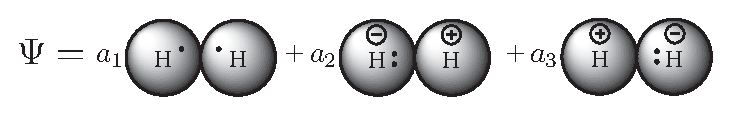
\includegraphics[scale=0.95]{figures/heitlerplus.eps}
  \end{center}
  \begin{equation*}
    \Psi= N \{ a_1(|1s_{A}\overline{1s_{B}}| - |\overline{1s_{A}}1s_{B}|) + a_2 |1s_{A}\overline{1s_{A}}| + a_3 |1s_{B}\overline{1s_{B}}| \}
  \end{equation*}
  \begin{itemize}
  \item<1-> Versatility is added by expanding with more structures
  \item<2-> $a_2 = a_3$, for homonuclear diatomic molecules
  \item<3-> Heteronuclear - ionic contribution will differ ($a_2 \neq a_3$)
  \end{itemize}
\end{frame}

\begin{frame}
  \frametitle{Coulson-Fischer Type Wave Function}
  \begin{center}  
    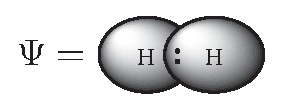
\includegraphics{figures/coulson.eps}
  \end{center}
  \begin{equation*}
    \Psi = N \{ | \phi_1 \overline{\phi_2} | - | \overline{\phi_1} \phi_2 | \}
  \end{equation*}
  \begin{center}
    where $\phi_1 = 1s_A + \lambda_1 1s_B$ and $\phi_2 = 1s_B + \lambda_2 1s_A$
  \end{center}  
  \begin{itemize}
    \item<1-> Introduced by Coulson and Fischer in 1949
    \item<2-> CF orbitals are spread over atoms (unless $\lambda$'s are zero)
    \item<3-> For polar diatomic molecules, the $\lambda$'s will differ
  \end{itemize}
\end{frame}

\begin{frame}
  \frametitle{Modern Valence Bond Wave Functions}
  \begin{columns}[c]
  \column{2in}
    \begin{equation*}
      \Psi = \sum_{i} C_i \Phi_i
    \end{equation*}

    \begin{equation*}
      \Phi = \sum_{i} \alpha_i \Delta_i
    \end{equation*}

    \begin{equation*}
      \Delta = |ijkl \cdots n|
    \end{equation*}

    \begin{equation*}
      i = \sum_{n} c_n \chi_n
    \end{equation*}
  \column{2in}
    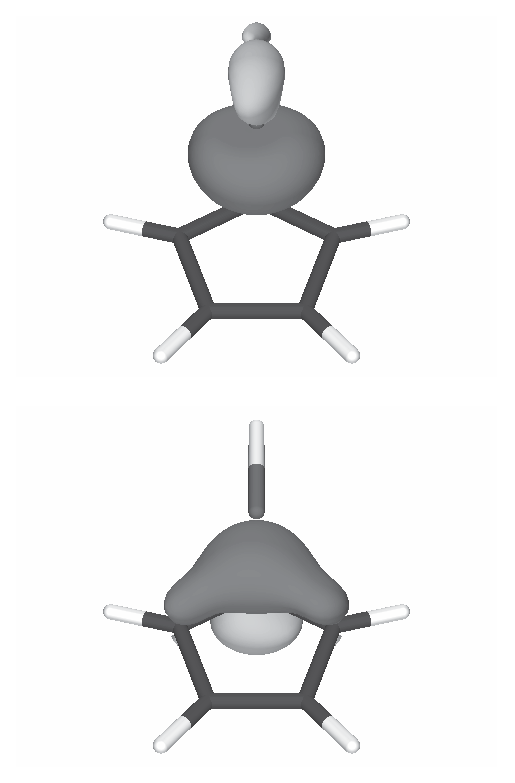
\includegraphics[scale=0.5]{figures/sigma_sih.eps}
  \end{columns}
\end{frame}

\subsection{Super-CI / Orbital Optimization}

\begin{frame}
  \frametitle{Simple slide with three points shown in succession}   % Insert frame title between curly braces

  \begin{itemize}
  \item<1-> Point 1 (Click ``Next Page'' to see Point 2) % Use Next Page to go to Point 2
  \item<2-> Point 2  % Use Next Page to go to Point 3
  \item<3-> Point 3
  \end{itemize}
\end{frame}

\section{Slide with two columns: items and a graphic}
\begin{frame}
  \frametitle{Slide with two columns: items and a graphic}   % Insert frame title between curly braces
  \begin{columns}[c]
  \column{2in}  % slides are 3in high by 5in wide
  \begin{itemize}
  \item<1-> First item
  \item<2-> Second item
  \item<3-> ...
  \end{itemize}
  \column{2in}
  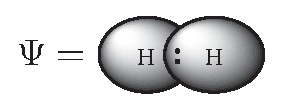
\includegraphics[height=0.5in]{figures/coulson.eps}
  \end{columns}
\end{frame}

\end{document}
